\clearpage
\SourceLeaf{170}
\begin{center}
EINIGE SÄTZE\\
DIE ERSTEN GRÜNDE DER GEOMETRIE BETREFFEND.
\end{center}

\medskip
\begin{center}
\rule{0.15\textwidth}{0.4pt}
\end{center}
\medskip

1) Parallellinie mit einer Geraden heisst die, von welcher die
Senkrechten auf letztere überall von gleicher Grösse sind.

2) Ob die Parallellinie selbst gerade ist, bleibt noch unentschieden.

3) $AB$ gerade, [$AC$ senkrecht auf $AB$,] $CD$ mit ihr parallel;
$AE$ gerade, unter gegebenem Winkel $BAE$, wird weit genug fortgesetzt
gewiss $CD$ schneiden. Beweis so zu führen:

\begin{center}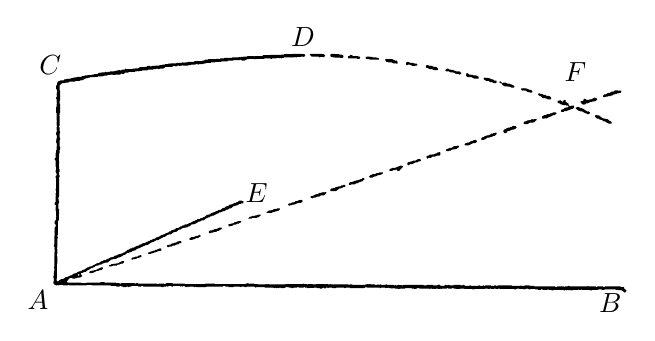
\begin{tikzpicture}[x=0.00572246cm,y=-0.00572246cm]
\fill[even odd rule] (208,578) -- (207,577) -- (204,577) -- (192,583) -- (189,583) -- (188,584) -- (185,584) -- (184,585) -- (180,585) -- (178,587) -- (178,589) -- (179,590) -- (182,590) -- (183,589) -- (186,589) -- (194,585) -- (197,585) -- (201,583) -- (205,583) -- (208,580) -- cycle
(255,564) -- (254,563) -- (251,563) -- (241,568) -- (227,570) -- (224,572) -- (222,572) -- (221,574) -- (222,575) -- (228,575) -- (231,573) -- (239,573) -- (241,571) -- (244,571) -- (248,569) -- (252,569) -- (254,567) -- cycle
(294,552) -- (292,550) -- (290,550) -- (289,551) -- (287,551) -- (285,553) -- (281,553) -- (277,555) -- (274,555) -- (272,557) -- (271,557) -- (271,559) -- (272,560) -- (274,560) -- (275,559) -- (282,558) -- (284,556) -- (288,556) -- (289,555) -- (291,555) -- cycle
(338,537) -- (336,535) -- (334,535) -- (327,538) -- (324,538) -- (323,540) -- (320,540) -- (319,541) -- (314,542) -- (311,544) -- (309,544) -- (308,546) -- (309,547) -- (314,547) -- (315,546) -- (318,546) -- (319,545) -- (321,545) -- (322,544) -- (324,544) -- (331,541) -- (337,540) -- (338,539) -- cycle
(382,520) -- (381,519) -- (376,519) -- (375,520) -- (373,520) -- (371,522) -- (368,522) -- (364,524) -- (361,524) -- (359,526) -- (351,528) -- (350,530) -- (352,532) -- (354,532) -- (355,531) -- (360,531) -- (363,529) -- (366,529) -- (372,526) -- (376,526) -- (376,525) -- (378,523) -- (382,523) -- cycle
(425,507) -- (423,505) -- (422,505) -- (419,507) -- (416,507) -- (409,510) -- (404,510) -- (400,513) -- (400,515) -- (401,516) -- (406,516) -- (407,515) -- (410,515) -- (415,512) -- (419,512) -- (421,510) -- (423,510) -- (425,508) -- cycle
(472,490) -- (471,489) -- (466,489) -- (460,492) -- (457,492) -- (450,495) -- (446,495) -- (443,497) -- (443,500) -- (444,501) -- (448,501) -- (449,500) -- (452,500) -- (455,498) -- (460,498) -- (462,496) -- (465,496) -- (467,494) -- (470,493) -- (472,491) -- cycle
(515,475) -- (514,474) -- (506,475) -- (505,476) -- (500,477) -- (498,479) -- (492,480) -- (491,481) -- (488,481) -- (486,483) -- (488,485) -- (488,486) -- (490,486) -- (491,485) -- (495,485) -- (498,482) -- (503,482) -- (506,480) -- (509,480) -- (512,478) -- (514,478) -- (515,477) -- cycle
(558,460) -- (553,460) -- (552,461) -- (546,462) -- (545,463) -- (539,463) -- (538,464) -- (534,465) -- (531,468) -- (531,469) -- (537,469) -- (540,467) -- (549,467) -- (550,466) -- (553,466) -- (558,462) -- cycle
(601,447) -- (600,446) -- (595,446) -- (594,447) -- (587,448) -- (584,450) -- (576,451) -- (571,455) -- (572,456) -- (583,456) -- (584,455) -- (598,451) -- (600,449) -- (601,449) -- cycle
(651,429) -- (648,427) -- (646,428) -- (643,428) -- (639,430) -- (636,430) -- (632,433) -- (628,433) -- (625,435) -- (622,435) -- (620,436) -- (619,438) -- (621,440) -- (623,440) -- (624,439) -- (627,439) -- (628,438) -- (632,438) -- (641,434) -- (647,434) -- (651,431) -- cycle
(704,411) -- (703,410) -- (701,410) -- (700,411) -- (696,410) -- (695,411) -- (688,412) -- (686,414) -- (680,415) -- (679,416) -- (677,416) -- (675,418) -- (670,419) -- (669,420) -- (669,422) -- (673,424) -- (676,422) -- (680,422) -- (684,420) -- (688,420) -- (692,417) -- (699,417) -- (704,412) -- cycle
(746,395) -- (745,394) -- (742,394) -- (741,395) -- (738,395) -- (735,397) -- (731,397) -- (730,398) -- (725,399) -- (722,401) -- (715,402) -- (713,404) -- (713,407) -- (714,408) -- (725,408) -- (733,402) -- (739,401) -- (741,399) -- (744,399) -- (746,397) -- cycle
(789,381) -- (787,379) -- (784,379) -- (782,381) -- (780,381) -- (777,383) -- (774,383) -- (773,384) -- (770,384) -- (769,385) -- (767,385) -- (760,388) -- (757,388) -- (754,390) -- (754,393) -- (755,394) -- (758,394) -- (759,393) -- (767,393) -- (769,391) -- (774,390) -- (776,388) -- (779,388) -- (780,387) -- (784,386) -- (788,382) -- (789,382) -- cycle
(830,367) -- (829,366) -- (822,366) -- (821,367) -- (815,368) -- (812,370) -- (807,370) -- (804,372) -- (802,372) -- (799,375) -- (799,376) -- (801,378) -- (806,378) -- (807,377) -- (809,377) -- (811,375) -- (814,375) -- (817,373) -- (826,371) -- (828,369) -- (829,369) -- cycle
(874,353) -- (871,351) -- (869,351) -- (857,356) -- (851,356) -- (850,357) -- (846,358) -- (844,360) -- (844,362) -- (845,363) -- (850,363) -- (852,361) -- (857,361) -- (858,360) -- (860,360) -- (862,363) -- (866,363) -- (867,361) -- (874,354) -- cycle
(914,339) -- (912,337) -- (907,337) -- (902,340) -- (897,340) -- (896,341) -- (885,344) -- (884,345) -- (884,349) -- (885,350) -- (888,350) -- (889,348) -- (894,348) -- (902,344) -- (906,344) -- (908,342) -- (911,342) -- (913,341) -- cycle
(957,322) -- (955,321) -- (954,322) -- (951,322) -- (949,324) -- (947,324) -- (943,326) -- (940,326) -- (939,327) -- (933,327) -- (931,329) -- (929,329) -- (926,331) -- (927,335) -- (928,336) -- (930,334) -- (936,334) -- (939,331) -- (945,331) -- (949,329) -- (955,329) -- (957,327) -- cycle
(998,308) -- (997,307) -- (994,307) -- (993,308) -- (987,308) -- (985,310) -- (981,312) -- (977,312) -- (974,314) -- (972,314) -- (970,316) -- (970,318) -- (971,319) -- (976,319) -- (977,318) -- (980,318) -- (982,316) -- (993,314) -- (998,310) -- cycle
(1038,297) -- (1036,294) -- (1030,295) -- (1028,297) -- (1025,297) -- (1020,300) -- (1017,300) -- (1016,301) -- (1012,302) -- (1011,303) -- (1011,305) -- (1012,306) -- (1020,306) -- (1030,301) -- (1034,301) -- (1036,300) -- (1038,298) -- cycle
(1082,279) -- (1081,278) -- (1079,278) -- (1078,279) -- (1075,279) -- (1074,280) -- (1070,280) -- (1067,283) -- (1065,283) -- (1064,284) -- (1060,284) -- (1057,286) -- (1055,286) -- (1053,288) -- (1051,288) -- (1048,290) -- (1048,294) -- (1053,294) -- (1059,291) -- (1061,289) -- (1066,289) -- (1067,288) -- (1072,287) -- (1075,285) -- (1078,285) -- (1082,281) -- cycle
(1126,266) -- (1123,263) -- (1118,263) -- (1114,266) -- (1112,266) -- (1111,267) -- (1107,267) -- (1099,271) -- (1097,273) -- (1097,276) -- (1099,279) -- (1103,279) -- (1107,274) -- (1111,274) -- (1114,272) -- (1120,271) -- (1124,269) -- (1126,267) -- cycle
(1171,249) -- (1170,248) -- (1165,248) -- (1164,249) -- (1160,248) -- (1157,250) -- (1150,251) -- (1147,253) -- (1144,253) -- (1142,256) -- (1142,258) -- (1143,259) -- (1151,259) -- (1155,256) -- (1162,256) -- (1163,255) -- (1165,255) -- (1169,251) -- (1170,251) -- cycle
(1300,241) -- (1300,242) -- (1305,247) -- (1308,247) -- (1311,249) -- (1316,250) -- (1319,253) -- (1323,253) -- (1325,255) -- (1331,258) -- (1336,258) -- (1337,257) -- (1337,254) -- (1333,252) -- (1328,248) -- (1324,248) -- (1323,247) -- (1317,246) -- (1309,240) -- (1302,239) -- cycle
(1215,235) -- (1213,233) -- (1208,233) -- (1204,235) -- (1201,235) -- (1199,237) -- (1194,237) -- (1191,239) -- (1188,239) -- (1183,242) -- (1183,246) -- (1184,247) -- (1194,246) -- (1199,243) -- (1203,242) -- (1207,239) -- (1211,239) -- (1213,237) -- (1214,237) -- cycle
(1257,223) -- (1257,224) -- (1263,229) -- (1267,230) -- (1268,231) -- (1272,231) -- (1279,235) -- (1281,235) -- (1283,237) -- (1286,237) -- (1289,235) -- (1289,233) -- (1286,231) -- (1283,231) -- (1272,224) -- (1267,223) -- (1264,221) -- (1261,221) -- cycle
(1217,208) -- (1217,211) -- (1220,213) -- (1222,213) -- (1224,215) -- (1226,215) -- (1229,217) -- (1236,217) -- (1237,218) -- (1240,218) -- (1241,219) -- (1241,221) -- (1240,222) -- (1236,222) -- (1235,223) -- (1233,223) -- (1230,226) -- (1226,227) -- (1225,228) -- (1225,231) -- (1226,232) -- (1230,232) -- (1233,230) -- (1237,230) -- (1241,228) -- (1244,228) -- (1246,226) -- (1251,225) -- (1254,222) -- (1254,219) -- (1253,218) -- (1248,218) -- (1247,219) -- (1244,219) -- (1242,217) -- (1241,213) -- (1237,211) -- (1235,209) -- (1235,206) -- (1234,205) -- (1232,205) -- (1229,209) -- (1227,209) -- (1223,206) -- (1221,207) -- (1218,207) -- cycle
(1305,203) -- (1304,202) -- (1302,202) -- (1300,200) -- (1292,204) -- (1288,204) -- (1287,205) -- (1284,205) -- (1283,206) -- (1282,206) -- (1279,203) -- (1275,203) -- (1275,206) -- (1272,208) -- (1269,208) -- (1268,210) -- (1272,215) -- (1276,216) -- (1277,215) -- (1279,215) -- (1280,213) -- (1284,213) -- (1290,210) -- (1301,208) -- (1305,205) -- cycle
(1174,193) -- (1175,195) -- (1181,198) -- (1184,201) -- (1192,202) -- (1195,204) -- (1202,204) -- (1203,203) -- (1203,200) -- (1199,197) -- (1192,196) -- (1189,194) -- (1186,194) -- (1183,192) -- (1179,192) -- (1178,191) -- (1176,191) -- cycle
(1359,186) -- (1358,185) -- (1345,184) -- (1341,187) -- (1337,187) -- (1333,190) -- (1329,190) -- (1324,193) -- (1321,193) -- (1319,195) -- (1318,198) -- (1319,199) -- (1323,199) -- (1324,198) -- (1328,198) -- (1329,197) -- (1334,197) -- (1335,196) -- (1340,195) -- (1342,193) -- (1344,193) -- (1345,192) -- (1348,192) -- (1349,191) -- (1352,191) -- (1353,190) -- (1357,190) -- cycle
(1136,181) -- (1136,182) -- (1139,185) -- (1143,184) -- (1144,185) -- (1147,185) -- (1151,188) -- (1155,188) -- (1156,189) -- (1160,189) -- (1161,188) -- (1161,186) -- (1158,183) -- (1155,183) -- (1148,180) -- (1144,180) -- (1142,179) -- (1141,180) -- (1137,180) -- cycle
(1088,165) -- (1088,166) -- (1090,168) -- (1092,168) -- (1094,170) -- (1094,171) -- (1099,175) -- (1111,176) -- (1115,178) -- (1120,178) -- (1121,177) -- (1121,175) -- (1119,173) -- (1115,171) -- (1113,171) -- (1110,169) -- (1105,169) -- (1102,167) -- (1097,167) -- (1096,168) -- (1094,168) -- (1090,164) -- cycle
(1053,158) -- (1053,159) -- (1056,162) -- (1058,162) -- (1059,163) -- (1064,163) -- (1067,166) -- (1072,166) -- (1074,168) -- (1080,168) -- (1082,166) -- (1082,163) -- (1076,162) -- (1074,160) -- (1072,160) -- (1065,157) -- (1055,156) -- cycle
(1014,148) -- (1014,152) -- (1018,155) -- (1026,155) -- (1032,158) -- (1042,158) -- (1042,154) -- (1036,151) -- (1030,151) -- (1029,150) -- (1026,150) -- (1025,149) -- (1021,149) -- (1017,146) -- (1016,146) -- cycle
(968,139) -- (968,140) -- (970,142) -- (976,142) -- (979,144) -- (984,144) -- (985,145) -- (988,145) -- (990,147) -- (998,148) -- (999,149) -- (1001,149) -- (1004,146) -- (999,142) -- (992,142) -- (985,139) -- (977,138) -- (974,136) -- (972,136) -- cycle
(925,130) -- (925,133) -- (926,134) -- (928,134) -- (933,137) -- (939,137) -- (942,139) -- (951,139) -- (952,138) -- (952,136) -- (948,132) -- (942,132) -- (939,130) -- (936,130) -- (935,129) -- (932,130) -- (930,128) -- (927,128) -- cycle
(881,123) -- (881,127) -- (882,128) -- (884,128) -- (885,127) -- (889,127) -- (895,130) -- (901,130) -- (902,129) -- (905,129) -- (906,128) -- (906,127) -- (904,125) -- (901,125) -- (900,124) -- (897,124) -- (896,123) -- (890,123) -- (886,121) -- (883,121) -- cycle
(835,115) -- (835,118) -- (837,120) -- (837,121) -- (841,121) -- (842,122) -- (849,122) -- (852,124) -- (858,124) -- (859,125) -- (861,125) -- (862,124) -- (862,121) -- (860,118) -- (857,118) -- (850,115) -- (838,115) -- (837,114) -- cycle
(791,111) -- (791,113) -- (792,114) -- (794,114) -- (795,115) -- (800,115) -- (801,116) -- (820,116) -- (821,115) -- (821,114) -- (819,112) -- (816,112) -- (815,111) -- (807,111) -- (806,110) -- (801,110) -- (800,109) -- (794,109) -- cycle
(752,108) -- (752,112) -- (753,113) -- (772,113) -- (773,114) -- (777,114) -- (779,112) -- (779,110) -- (778,109) -- (775,109) -- (774,108) -- (763,108) -- (761,106) -- (757,106) -- (755,108) -- cycle
(713,105) -- (713,108) -- (715,110) -- (717,110) -- (718,111) -- (740,112) -- (742,110) -- (741,106) -- (739,106) -- (738,105) -- (733,105) -- (732,104) -- (723,104) -- (722,103) -- (715,103) -- cycle
(667,105) -- (671,109) -- (686,109) -- (688,111) -- (690,111) -- (691,110) -- (696,110) -- (697,111) -- (701,108) -- (701,106) -- (698,104) -- (695,104) -- (694,103) -- (669,103) -- cycle
(104,174) -- (104,180) -- (106,183) -- (106,186) -- (107,187) -- (106,188) -- (106,191) -- (105,192) -- (106,198) -- (104,200) -- (104,202) -- (105,203) -- (105,207) -- (106,208) -- (105,210) -- (106,214) -- (105,215) -- (105,221) -- (104,222) -- (104,233) -- (105,234) -- (105,240) -- (106,241) -- (105,242) -- (105,250) -- (106,251) -- (106,253) -- (105,254) -- (105,261) -- (106,262) -- (106,265) -- (105,266) -- (105,271) -- (106,272) -- (106,275) -- (104,279) -- (104,282) -- (106,285) -- (106,290) -- (105,291) -- (104,299) -- (105,300) -- (105,303) -- (106,304) -- (106,308) -- (105,309) -- (105,317) -- (104,318) -- (104,322) -- (103,323) -- (103,331) -- (104,332) -- (101,336) -- (101,338) -- (103,340) -- (103,353) -- (104,354) -- (104,361) -- (103,362) -- (103,365) -- (105,369) -- (105,373) -- (103,375) -- (103,378) -- (104,379) -- (104,402) -- (103,403) -- (103,406) -- (104,407) -- (104,412) -- (103,413) -- (103,416) -- (104,418) -- (103,419) -- (103,432) -- (101,434) -- (101,437) -- (104,440) -- (104,442) -- (103,443) -- (103,451) -- (104,452) -- (104,463) -- (105,465) -- (104,466) -- (104,471) -- (101,475) -- (101,480) -- (103,482) -- (103,487) -- (101,489) -- (101,497) -- (100,498) -- (101,500) -- (101,506) -- (100,507) -- (100,526) -- (99,527) -- (99,530) -- (101,533) -- (101,535) -- (100,536) -- (101,537) -- (101,544) -- (100,545) -- (101,549) -- (100,550) -- (100,576) -- (99,577) -- (100,579) -- (100,585) -- (99,586) -- (99,595) -- (98,596) -- (98,600) -- (99,601) -- (99,608) -- (98,609) -- (98,612) -- (100,615) -- (104,617) -- (106,617) -- (107,616) -- (109,617) -- (111,616) -- (119,616) -- (120,617) -- (130,617) -- (131,616) -- (133,616) -- (134,617) -- (149,617) -- (150,616) -- (152,617) -- (171,617) -- (172,616) -- (182,616) -- (183,617) -- (225,617) -- (226,618) -- (237,618) -- (239,620) -- (244,620) -- (246,618) -- (248,618) -- (250,620) -- (253,620) -- (254,621) -- (259,621) -- (260,620) -- (264,620) -- (265,621) -- (266,620) -- (270,620) -- (272,618) -- (286,618) -- (288,620) -- (292,620) -- (294,618) -- (297,618) -- (298,620) -- (337,620) -- (338,621) -- (341,621) -- (342,620) -- (347,620) -- (349,618) -- (351,620) -- (352,620) -- (354,618) -- (359,618) -- (361,620) -- (363,620) -- (364,618) -- (379,618) -- (381,620) -- (383,618) -- (385,620) -- (387,618) -- (388,618) -- (392,621) -- (395,621) -- (396,620) -- (398,620) -- (399,621) -- (400,620) -- (409,620) -- (410,621) -- (412,621) -- (413,620) -- (415,620) -- (416,621) -- (436,621) -- (437,620) -- (474,620) -- (476,618) -- (479,618) -- (481,620) -- (487,620) -- (488,621) -- (497,621) -- (498,620) -- (512,620) -- (513,621) -- (515,620) -- (522,620) -- (523,621) -- (526,621) -- (527,620) -- (544,620) -- (546,622) -- (548,621) -- (567,621) -- (568,622) -- (586,622) -- (587,623) -- (589,623) -- (590,622) -- (592,623) -- (594,623) -- (595,622) -- (597,623) -- (599,623) -- (600,622) -- (602,622) -- (603,623) -- (608,623) -- (610,622) -- (611,623) -- (614,621) -- (620,621) -- (621,622) -- (626,622) -- (627,623) -- (630,623) -- (631,622) -- (638,622) -- (639,621) -- (642,621) -- (643,622) -- (653,622) -- (654,621) -- (656,621) -- (657,622) -- (661,622) -- (662,623) -- (682,622) -- (683,623) -- (689,623) -- (690,624) -- (694,624) -- (697,622) -- (698,622) -- (700,624) -- (701,624) -- (703,622) -- (707,622) -- (708,623) -- (709,622) -- (717,622) -- (718,623) -- (725,623) -- (726,622) -- (743,622) -- (744,623) -- (746,623) -- (747,622) -- (756,622) -- (757,623) -- (788,623) -- (791,621) -- (793,621) -- (794,622) -- (822,622) -- (823,623) -- (825,623) -- (826,622) -- (834,622) -- (835,623) -- (842,622) -- (843,623) -- (848,623) -- (849,624) -- (855,623) -- (856,624) -- (862,624) -- (863,625) -- (866,625) -- (867,624) -- (878,624) -- (879,623) -- (893,623) -- (894,624) -- (898,624) -- (899,625) -- (905,624) -- (906,623) -- (910,623) -- (911,624) -- (932,624) -- (933,625) -- (935,624) -- (938,624) -- (939,625) -- (941,625) -- (942,624) -- (944,625) -- (947,625) -- (948,624) -- (956,625) -- (958,624) -- (960,625) -- (961,624) -- (971,624) -- (972,623) -- (974,623) -- (975,624) -- (982,624) -- (983,623) -- (986,623) -- (987,624) -- (991,624) -- (992,625) -- (1010,624) -- (1011,625) -- (1028,625) -- (1029,626) -- (1032,626) -- (1033,625) -- (1055,625) -- (1056,624) -- (1062,624) -- (1063,625) -- (1066,625) -- (1067,624) -- (1069,624) -- (1070,625) -- (1075,625) -- (1076,624) -- (1084,625) -- (1085,624) -- (1088,624) -- (1089,625) -- (1120,625) -- (1121,626) -- (1125,626) -- (1127,624) -- (1132,624) -- (1133,625) -- (1141,625) -- (1142,626) -- (1144,626) -- (1145,625) -- (1150,624) -- (1154,626) -- (1156,626) -- (1157,625) -- (1167,625) -- (1168,626) -- (1173,626) -- (1174,627) -- (1179,627) -- (1180,626) -- (1184,626) -- (1185,627) -- (1194,627) -- (1195,626) -- (1197,626) -- (1198,627) -- (1203,627) -- (1204,628) -- (1207,628) -- (1208,627) -- (1230,627) -- (1231,628) -- (1233,628) -- (1234,627) -- (1236,627) -- (1237,628) -- (1239,627) -- (1241,627) -- (1242,628) -- (1246,627) -- (1247,628) -- (1250,628) -- (1251,627) -- (1262,627) -- (1263,626) -- (1265,627) -- (1269,627) -- (1271,626) -- (1272,627) -- (1288,627) -- (1289,628) -- (1293,628) -- (1294,627) -- (1307,627) -- (1308,626) -- (1315,626) -- (1316,627) -- (1321,627) -- (1322,626) -- (1346,626) -- (1347,627) -- (1360,628) -- (1366,633) -- (1367,633) -- (1370,629) -- (1370,628) -- (1365,624) -- (1365,622) -- (1364,621) -- (1358,621) -- (1356,619) -- (1323,619) -- (1321,621) -- (1320,621) -- (1318,619) -- (1306,619) -- (1304,621) -- (1303,621) -- (1301,619) -- (1285,619) -- (1284,618) -- (1283,619) -- (1244,619) -- (1243,618) -- (1241,618) -- (1240,619) -- (1234,619) -- (1232,621) -- (1230,619) -- (1217,619) -- (1215,621) -- (1213,621) -- (1211,619) -- (1165,619) -- (1164,618) -- (1155,618) -- (1154,617) -- (1145,617) -- (1144,618) -- (1137,618) -- (1136,617) -- (1134,618) -- (1116,618) -- (1115,617) -- (1085,617) -- (1084,618) -- (1081,618) -- (1080,617) -- (1077,617) -- (1076,618) -- (1070,618) -- (1069,617) -- (1057,617) -- (1056,618) -- (1054,618) -- (1053,617) -- (1051,618) -- (1045,618) -- (1044,617) -- (1042,617) -- (1041,618) -- (1025,618) -- (1024,617) -- (1022,617) -- (1021,618) -- (1012,618) -- (1009,616) -- (1007,616) -- (1006,617) -- (1002,617) -- (1001,616) -- (987,616) -- (986,617) -- (978,617) -- (977,616) -- (974,616) -- (973,617) -- (971,617) -- (970,616) -- (968,616) -- (966,618) -- (958,618) -- (954,615) -- (950,617) -- (941,617) -- (940,616) -- (927,616) -- (926,617) -- (920,617) -- (919,616) -- (875,616) -- (874,617) -- (863,616) -- (862,617) -- (858,617) -- (857,616) -- (856,617) -- (854,617) -- (853,616) -- (839,616) -- (838,615) -- (836,615) -- (835,616) -- (826,616) -- (825,615) -- (812,616) -- (811,615) -- (802,615) -- (801,614) -- (799,614) -- (798,615) -- (795,614) -- (794,615) -- (791,615) -- (790,616) -- (762,616) -- (761,615) -- (756,615) -- (754,616) -- (753,615) -- (714,615) -- (713,614) -- (711,615) -- (708,615) -- (707,614) -- (702,614) -- (701,615) -- (699,614) -- (681,614) -- (680,615) -- (674,615) -- (673,614) -- (664,614) -- (663,615) -- (661,615) -- (660,614) -- (654,614) -- (653,613) -- (651,614) -- (614,614) -- (613,615) -- (577,615) -- (576,614) -- (574,614) -- (573,615) -- (571,615) -- (570,614) -- (568,615) -- (552,615) -- (551,614) -- (544,614) -- (543,613) -- (531,613) -- (530,612) -- (528,613) -- (525,613) -- (524,614) -- (457,614) -- (456,613) -- (436,613) -- (435,614) -- (390,614) -- (389,613) -- (363,613) -- (362,612) -- (349,612) -- (346,614) -- (344,614) -- (343,613) -- (332,613) -- (331,614) -- (329,614) -- (328,613) -- (286,613) -- (285,612) -- (282,612) -- (281,613) -- (279,613) -- (278,612) -- (249,612) -- (248,613) -- (245,613) -- (244,612) -- (238,612) -- (237,611) -- (212,611) -- (211,610) -- (203,610) -- (202,611) -- (172,611) -- (171,612) -- (160,612) -- (159,611) -- (130,611) -- (128,609) -- (128,608) -- (134,601) -- (139,600) -- (141,602) -- (146,602) -- (147,601) -- (150,601) -- (151,600) -- (156,600) -- (157,599) -- (159,599) -- (162,596) -- (162,595) -- (159,593) -- (159,590) -- (160,589) -- (163,589) -- (167,587) -- (170,587) -- (173,584) -- (179,581) -- (181,579) -- (184,579) -- (186,577) -- (188,577) -- (190,575) -- (194,573) -- (197,573) -- (200,571) -- (204,571) -- (208,568) -- (210,568) -- (211,567) -- (219,566) -- (226,560) -- (228,560) -- (232,558) -- (237,558) -- (240,556) -- (247,554) -- (251,552) -- (253,550) -- (257,549) -- (262,545) -- (265,545) -- (266,544) -- (271,543) -- (273,541) -- (280,539) -- (282,537) -- (286,535) -- (288,535) -- (293,532) -- (295,532) -- (297,530) -- (299,530) -- (302,528) -- (308,527) -- (313,523) -- (317,521) -- (319,521) -- (326,517) -- (332,516) -- (334,514) -- (339,512) -- (341,510) -- (346,509) -- (351,505) -- (353,505) -- (354,504) -- (358,504) -- (365,499) -- (371,498) -- (377,493) -- (380,493) -- (384,490) -- (395,488) -- (398,486) -- (400,486) -- (404,482) -- (411,481) -- (417,478) -- (419,476) -- (424,475) -- (427,473) -- (431,473) -- (436,469) -- (442,466) -- (444,466) -- (446,464) -- (448,464) -- (451,462) -- (454,462) -- (461,458) -- (463,458) -- (466,455) -- (469,455) -- (475,452) -- (478,452) -- (482,449) -- (485,449) -- (489,446) -- (492,446) -- (498,441) -- (501,441) -- (502,440) -- (507,439) -- (511,436) -- (514,436) -- (515,435) -- (520,435) -- (520,430) -- (517,430) -- (516,429) -- (511,429) -- (507,432) -- (505,432) -- (503,434) -- (500,434) -- (495,437) -- (489,438) -- (487,440) -- (481,442) -- (478,445) -- (475,445) -- (468,450) -- (464,450) -- (462,452) -- (459,452) -- (457,454) -- (450,456) -- (444,460) -- (441,460) -- (437,462) -- (434,465) -- (432,465) -- (430,467) -- (425,468) -- (422,470) -- (418,470) -- (416,472) -- (414,472) -- (412,474) -- (410,474) -- (401,479) -- (399,479) -- (397,481) -- (390,482) -- (387,484) -- (385,484) -- (383,486) -- (380,486) -- (378,488) -- (374,490) -- (371,490) -- (367,493) -- (360,495) -- (358,497) -- (356,497) -- (354,499) -- (350,501) -- (348,501) -- (346,503) -- (339,505) -- (335,507) -- (333,509) -- (328,510) -- (322,514) -- (319,514) -- (317,516) -- (314,516) -- (312,518) -- (310,518) -- (308,520) -- (306,520) -- (301,523) -- (295,524) -- (293,526) -- (289,527) -- (287,529) -- (282,530) -- (277,533) -- (274,533) -- (272,535) -- (269,535) -- (265,538) -- (263,538) -- (256,544) -- (254,544) -- (251,546) -- (243,548) -- (237,551) -- (234,551) -- (231,554) -- (225,555) -- (220,558) -- (218,558) -- (214,561) -- (210,561) -- (208,563) -- (206,563) -- (202,565) -- (200,567) -- (195,568) -- (182,575) -- (179,575) -- (176,577) -- (174,577) -- (167,582) -- (165,582) -- (158,586) -- (155,586) -- (148,590) -- (143,591) -- (138,595) -- (136,595) -- (130,598) -- (125,599) -- (123,601) -- (119,603) -- (116,603) -- (112,605) -- (109,608) -- (107,608) -- (105,606) -- (105,602) -- (106,601) -- (106,569) -- (107,568) -- (107,553) -- (106,552) -- (106,547) -- (107,546) -- (107,537) -- (106,536) -- (106,533) -- (107,532) -- (107,513) -- (108,512) -- (108,510) -- (107,509) -- (107,506) -- (108,505) -- (108,475) -- (110,472) -- (110,460) -- (111,459) -- (111,456) -- (110,455) -- (111,449) -- (109,447) -- (109,436) -- (111,433) -- (111,430) -- (110,429) -- (109,423) -- (111,419) -- (111,377) -- (112,376) -- (112,373) -- (111,372) -- (111,365) -- (112,364) -- (112,360) -- (111,359) -- (111,352) -- (110,351) -- (110,347) -- (111,346) -- (111,341) -- (110,340) -- (110,331) -- (111,330) -- (111,324) -- (112,323) -- (112,320) -- (111,318) -- (113,316) -- (113,310) -- (112,309) -- (112,295) -- (113,294) -- (113,290) -- (112,289) -- (112,280) -- (113,279) -- (113,276) -- (112,275) -- (112,267) -- (111,266) -- (111,263) -- (112,262) -- (112,242) -- (111,240) -- (112,239) -- (112,235) -- (113,234) -- (113,215) -- (112,214) -- (112,207) -- (113,206) -- (113,185) -- (112,184) -- (112,175) -- (111,174) -- (116,169) -- (118,168) -- (124,168) -- (125,167) -- (131,167) -- (133,165) -- (145,165) -- (148,163) -- (156,163) -- (157,162) -- (161,162) -- (171,157) -- (175,157) -- (176,156) -- (179,156) -- (180,155) -- (190,155) -- (191,154) -- (196,154) -- (197,153) -- (207,153) -- (208,152) -- (218,151) -- (219,150) -- (224,150) -- (225,149) -- (235,150) -- (236,149) -- (246,149) -- (249,147) -- (255,148) -- (255,147) -- (257,145) -- (263,145) -- (266,143) -- (279,143) -- (280,142) -- (283,142) -- (284,141) -- (288,142) -- (289,141) -- (294,141) -- (295,140) -- (306,140) -- (308,138) -- (319,138) -- (320,137) -- (326,137) -- (327,136) -- (330,136) -- (331,137) -- (333,137) -- (334,136) -- (341,136) -- (345,134) -- (347,132) -- (362,132) -- (364,130) -- (368,130) -- (369,131) -- (371,131) -- (374,129) -- (380,130) -- (381,129) -- (384,129) -- (385,128) -- (386,129) -- (397,129) -- (398,128) -- (403,128) -- (404,127) -- (413,127) -- (414,126) -- (418,126) -- (420,127) -- (421,126) -- (426,126) -- (427,125) -- (430,126) -- (431,125) -- (437,124) -- (438,123) -- (447,123) -- (448,122) -- (456,122) -- (457,121) -- (470,121) -- (471,120) -- (484,120) -- (486,118) -- (497,118) -- (498,117) -- (511,117) -- (513,116) -- (517,118) -- (522,118) -- (528,115) -- (532,115) -- (533,114) -- (541,114) -- (542,115) -- (550,115) -- (551,114) -- (566,114) -- (567,113) -- (579,113) -- (580,114) -- (583,114) -- (584,113) -- (593,113) -- (594,112) -- (605,113) -- (606,112) -- (609,112) -- (610,111) -- (632,111) -- (633,110) -- (638,111) -- (639,110) -- (647,110) -- (648,109) -- (652,109) -- (654,110) -- (657,107) -- (657,106) -- (655,104) -- (651,104) -- (650,103) -- (629,103) -- (628,104) -- (617,104) -- (615,103) -- (614,104) -- (610,104) -- (609,105) -- (564,106) -- (562,108) -- (545,108) -- (544,109) -- (542,108) -- (529,108) -- (528,109) -- (521,109) -- (520,110) -- (514,110) -- (513,111) -- (510,110) -- (509,111) -- (495,111) -- (494,112) -- (478,112) -- (477,113) -- (469,113) -- (468,114) -- (460,114) -- (459,115) -- (442,115) -- (441,116) -- (435,116) -- (432,118) -- (429,118) -- (428,119) -- (412,119) -- (410,121) -- (397,121) -- (396,122) -- (391,122) -- (390,123) -- (384,122) -- (383,123) -- (372,123) -- (371,124) -- (359,124) -- (358,125) -- (353,125) -- (352,126) -- (346,126) -- (345,127) -- (340,127) -- (339,128) -- (334,128) -- (333,129) -- (324,129) -- (323,130) -- (317,130) -- (316,131) -- (313,131) -- (312,130) -- (307,130) -- (305,132) -- (289,133) -- (287,135) -- (274,136) -- (273,137) -- (260,137) -- (258,136) -- (255,139) -- (254,138) -- (251,138) -- (248,140) -- (244,139) -- (243,140) -- (239,140) -- (238,141) -- (234,141) -- (233,142) -- (224,142) -- (223,143) -- (219,143) -- (218,144) -- (216,144) -- (215,143) -- (213,143) -- (212,144) -- (206,144) -- (205,145) -- (201,145) -- (200,146) -- (198,146) -- (196,148) -- (189,148) -- (188,149) -- (184,149) -- (183,150) -- (168,151) -- (167,152) -- (161,153) -- (160,154) -- (151,154) -- (150,155) -- (142,156) -- (141,157) -- (138,157) -- (137,158) -- (126,159) -- (125,160) -- (122,160) -- (121,162) -- (114,162) -- (113,163) -- (109,164) -- (107,166) -- (106,172) -- cycle
(154,591) -- (156,593) -- (156,594) -- (154,596) -- (152,594) -- (152,593) -- cycle;
\node[inner sep=0pt] at (652,66) {$D$};
\node[inner sep=0pt] at (91,127) {$C$};
\node[inner sep=0pt] at (1257,143) {$F$};
\node[inner sep=0pt] at (549,411) {$E$};
\node[inner sep=0pt] at (64,650) {$A$};
\node[inner sep=0pt] at (1334,657) {$B$};
\end{tikzpicture}
\end{center}

Es sei
\[
2^n > \frac{90^{0}}{BAE}, \qquad BAF = \frac{90^{0}}{2^n}, \qquad
AF \EqualsOverGreater{} 2^n AC, 
\]
so liegt gewiss $F$ jenseits $CD$, also schneidet $AF$ die $CD$ und
a potiori schneidet $AE$ die $CD$.

4) $BE$ und $AC$ auf $AB$ senkrecht, $CD$ parallel, $CE$ gerade.
[$ACE$ ein Rechter.] Falls $BEC$ \textls{stumpf} ist, wird $BE < AC$: alsdann
liegt $CE$ ganz unterhalb $CD$.

\begin{center}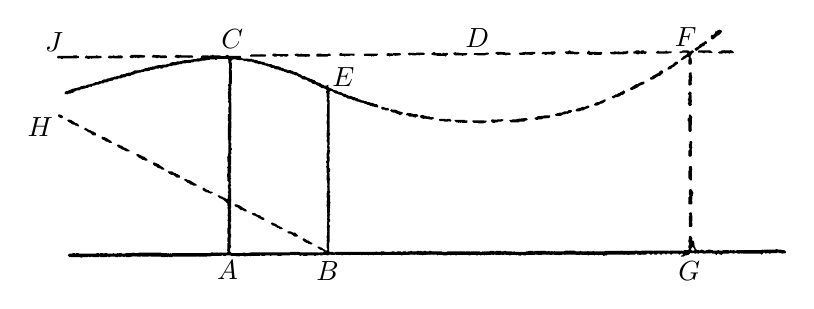
\begin{tikzpicture}[x=0.00564972cm,y=-0.00564972cm]
\fill[even odd rule] (1522,449) -- (1519,452) -- (1520,454) -- (1520,457) -- (1519,458) -- (1519,481) -- (1520,482) -- (1525,482) -- (1527,479) -- (1527,473) -- (1526,472) -- (1526,470) -- (1527,469) -- (1527,457) -- (1526,456) -- (1526,451) -- (1524,449) -- cycle
(1521,397) -- (1519,401) -- (1519,409) -- (1520,410) -- (1520,413) -- (1518,416) -- (1518,430) -- (1519,431) -- (1525,431) -- (1527,429) -- (1527,425) -- (1526,424) -- (1527,416) -- (1526,414) -- (1528,412) -- (1528,408) -- (1529,407) -- (1529,405) -- (1526,399) -- (1524,397) -- cycle
(425,395) -- (425,399) -- (433,404) -- (437,404) -- (439,406) -- (441,406) -- (442,407) -- (444,407) -- (448,405) -- (447,403) -- (441,402) -- (438,399) -- (434,398) -- (429,394) -- (426,394) -- cycle
(384,375) -- (384,377) -- (386,379) -- (387,379) -- (390,382) -- (395,384) -- (398,387) -- (401,387) -- (404,389) -- (411,389) -- (412,388) -- (411,386) -- (396,377) -- (391,376) -- (388,374) -- (385,374) -- cycle
(347,358) -- (347,359) -- (351,363) -- (355,365) -- (359,365) -- (367,371) -- (373,371) -- (374,370) -- (374,367) -- (372,365) -- (371,365) -- (369,363) -- (367,363) -- (365,361) -- (363,361) -- (359,359) -- (357,357) -- (348,357) -- cycle
(1521,345) -- (1519,347) -- (1519,355) -- (1518,356) -- (1518,372) -- (1522,377) -- (1525,377) -- (1526,376) -- (1526,361) -- (1525,359) -- (1526,358) -- (1526,354) -- (1527,352) -- (1526,351) -- (1526,347) -- (1524,345) -- cycle
(314,338) -- (314,342) -- (316,344) -- (321,346) -- (324,349) -- (331,351) -- (333,353) -- (338,353) -- (339,352) -- (339,351) -- (335,347) -- (334,347) -- (326,341) -- (317,337) -- (315,337) -- cycle
(276,319) -- (277,322) -- (284,328) -- (286,328) -- (290,331) -- (293,331) -- (296,333) -- (300,333) -- (301,332) -- (301,330) -- (294,324) -- (292,324) -- (280,318) -- (277,318) -- cycle
(233,298) -- (233,300) -- (237,304) -- (240,305) -- (244,308) -- (246,308) -- (253,312) -- (260,312) -- (261,311) -- (261,310) -- (259,308) -- (257,308) -- (255,306) -- (248,303) -- (243,299) -- (241,299) -- (238,297) -- (234,297) -- cycle
(1522,289) -- (1520,291) -- (1521,294) -- (1519,296) -- (1519,304) -- (1521,306) -- (1521,307) -- (1518,311) -- (1518,322) -- (1521,324) -- (1524,324) -- (1526,320) -- (1526,311) -- (1525,310) -- (1525,308) -- (1526,307) -- (1526,304) -- (1527,303) -- (1526,301) -- (1526,294) -- (1527,292) -- (1525,289) -- cycle
(198,280) -- (198,283) -- (201,286) -- (203,286) -- (208,290) -- (211,290) -- (213,292) -- (215,292) -- (216,293) -- (220,293) -- (221,292) -- (221,291) -- (217,287) -- (213,285) -- (210,282) -- (208,282) -- (205,280) -- (201,280) -- (200,279) -- cycle
(159,261) -- (159,263) -- (161,265) -- (163,265) -- (168,269) -- (172,270) -- (177,275) -- (179,276) -- (184,276) -- (185,275) -- (185,271) -- (183,269) -- (181,269) -- (179,267) -- (177,267) -- (172,264) -- (170,264) -- (162,259) -- (161,259) -- cycle
(1032,243) -- (1032,245) -- (1035,248) -- (1045,248) -- (1046,249) -- (1057,249) -- (1058,248) -- (1061,248) -- (1064,245) -- (1064,243) -- (1059,243) -- (1058,242) -- (1033,242) -- cycle
(992,242) -- (992,243) -- (996,247) -- (1000,247) -- (1001,248) -- (1002,247) -- (1004,247) -- (1005,248) -- (1007,247) -- (1009,247) -- (1010,248) -- (1019,248) -- (1021,246) -- (1021,243) -- (1020,242) -- (1015,242) -- (1014,241) -- (993,241) -- cycle
(121,242) -- (121,243) -- (125,247) -- (128,248) -- (130,250) -- (134,252) -- (137,252) -- (139,254) -- (141,254) -- (144,256) -- (146,256) -- (147,255) -- (147,253) -- (143,249) -- (139,248) -- (129,241) -- (126,241) -- (125,240) -- cycle
(1102,241) -- (1098,239) -- (1096,240) -- (1088,240) -- (1087,241) -- (1076,240) -- (1074,242) -- (1074,244) -- (1077,247) -- (1079,248) -- (1082,248) -- (1083,247) -- (1088,247) -- (1090,245) -- (1097,245) -- (1101,243) -- cycle
(957,240) -- (957,242) -- (959,244) -- (968,244) -- (969,245) -- (977,245) -- (978,244) -- (980,244) -- (981,245) -- (983,245) -- (985,243) -- (985,241) -- (984,241) -- (982,239) -- (975,239) -- (974,240) -- (972,240) -- (971,239) -- (958,239) -- cycle
(1156,239) -- (1153,237) -- (1147,237) -- (1146,238) -- (1141,238) -- (1140,239) -- (1137,238) -- (1136,239) -- (1132,239) -- (1131,240) -- (1122,240) -- (1121,241) -- (1116,241) -- (1115,243) -- (1119,247) -- (1136,247) -- (1138,245) -- (1149,245) -- (1151,243) -- (1155,242) -- (1156,241) -- cycle
(1207,232) -- (1206,231) -- (1193,231) -- (1192,232) -- (1179,233) -- (1177,235) -- (1173,236) -- (1172,237) -- (1172,239) -- (1173,239) -- (1175,241) -- (1179,241) -- (1180,240) -- (1187,240) -- (1191,238) -- (1204,237) -- (1207,235) -- cycle
(914,233) -- (914,234) -- (918,238) -- (920,238) -- (921,239) -- (927,238) -- (928,239) -- (933,239) -- (934,240) -- (938,240) -- (939,241) -- (945,239) -- (945,236) -- (944,235) -- (937,235) -- (935,233) -- (929,233) -- (928,232) -- (925,232) -- (921,230) -- (916,231) -- cycle
(1521,229) -- (1519,231) -- (1519,236) -- (1516,239) -- (1516,243) -- (1518,245) -- (1518,265) -- (1520,268) -- (1523,268) -- (1526,264) -- (1525,262) -- (1525,253) -- (1526,252) -- (1526,237) -- (1527,235) -- (1525,233) -- (1525,232) -- (1522,229) -- cycle
(100,230) -- (100,233) -- (105,237) -- (109,237) -- (111,235) -- (111,233) -- (107,230) -- (105,230) -- (104,229) -- (101,229) -- cycle
(883,228) -- (883,230) -- (884,231) -- (887,231) -- (890,234) -- (898,234) -- (899,235) -- (902,235) -- (903,236) -- (904,236) -- (906,234) -- (910,234) -- (910,230) -- (906,228) -- (899,228) -- (898,227) -- (895,227) -- (894,226) -- (888,226) -- (887,225) -- cycle
(1256,221) -- (1254,219) -- (1248,219) -- (1248,220) -- (1246,222) -- (1239,222) -- (1233,225) -- (1227,225) -- (1226,226) -- (1223,226) -- (1222,227) -- (1220,227) -- (1218,229) -- (1218,230) -- (1220,232) -- (1231,232) -- (1236,229) -- (1239,229) -- (1243,227) -- (1247,228) -- (1249,226) -- (1253,225) -- (1256,222) -- cycle
(847,220) -- (851,224) -- (853,224) -- (854,225) -- (858,225) -- (861,227) -- (865,228) -- (869,231) -- (871,229) -- (873,229) -- (875,227) -- (875,224) -- (864,221) -- (862,219) -- (860,219) -- (859,218) -- (852,218) -- (850,217) -- cycle
(827,213) -- (827,216) -- (829,218) -- (834,218) -- (836,220) -- (843,220) -- (844,218) -- (844,216) -- (841,214) -- (836,214) -- (832,212) -- (828,212) -- cycle
(1295,211) -- (1293,209) -- (1291,209) -- (1285,212) -- (1279,212) -- (1275,214) -- (1272,214) -- (1271,215) -- (1267,216) -- (1264,219) -- (1264,220) -- (1266,222) -- (1273,222) -- (1277,220) -- (1282,220) -- (1284,218) -- (1288,216) -- (1290,216) -- (1292,214) -- (1294,214) -- (1295,213) -- cycle
(1331,195) -- (1328,195) -- (1326,197) -- (1324,197) -- (1317,201) -- (1313,201) -- (1312,202) -- (1310,202) -- (1306,206) -- (1306,207) -- (1308,209) -- (1313,209) -- (1314,208) -- (1316,208) -- (1319,205) -- (1325,204) -- (1332,199) -- cycle
(1521,177) -- (1517,182) -- (1517,183) -- (1519,185) -- (1518,193) -- (1517,194) -- (1517,197) -- (1518,198) -- (1518,202) -- (1517,203) -- (1517,205) -- (1518,206) -- (1518,208) -- (1520,210) -- (1523,210) -- (1526,207) -- (1525,205) -- (1526,197) -- (1525,196) -- (1525,186) -- (1524,185) -- (1525,183) -- (1525,180) -- cycle
(1376,178) -- (1373,175) -- (1372,175) -- (1370,177) -- (1365,179) -- (1363,181) -- (1361,181) -- (1356,184) -- (1354,184) -- (1349,187) -- (1347,187) -- (1346,188) -- (1346,190) -- (1349,193) -- (1350,193) -- (1354,190) -- (1359,190) -- (1360,189) -- (1362,189) -- (1367,185) -- (1370,185) -- (1372,184) -- (1375,181) -- cycle
(1419,156) -- (1418,155) -- (1412,156) -- (1406,159) -- (1404,161) -- (1400,161) -- (1389,168) -- (1387,170) -- (1387,172) -- (1389,174) -- (1392,174) -- (1395,172) -- (1397,172) -- (1399,170) -- (1401,170) -- (1409,164) -- (1417,161) -- (1419,159) -- cycle
(1524,134) -- (1520,135) -- (1519,136) -- (1519,143) -- (1518,144) -- (1519,146) -- (1519,150) -- (1518,151) -- (1518,162) -- (1520,164) -- (1524,163) -- (1526,160) -- (1525,158) -- (1525,154) -- (1526,153) -- (1526,147) -- (1527,145) -- (1526,144) -- (1526,141) -- (1525,140) -- (1525,135) -- cycle
(1461,132) -- (1459,130) -- (1456,130) -- (1454,131) -- (1451,135) -- (1438,142) -- (1436,144) -- (1432,146) -- (1431,148) -- (1433,150) -- (1433,151) -- (1439,150) -- (1446,145) -- (1452,142) -- (1454,142) -- (1461,135) -- cycle
(1494,111) -- (1493,110) -- (1490,110) -- (1488,111) -- (1482,117) -- (1474,121) -- (1471,124) -- (1471,127) -- (1472,128) -- (1478,127) -- (1482,123) -- (1485,122) -- (1492,116) -- (1493,116) -- (1494,115) -- cycle
(212,101) -- (215,103) -- (221,103) -- (222,102) -- (225,102) -- (226,103) -- (243,103) -- (246,100) -- (246,99) -- (242,96) -- (240,96) -- (239,97) -- (237,96) -- (235,96) -- (234,97) -- (227,97) -- (226,96) -- (224,96) -- (223,97) -- (218,97) -- (217,96) -- (215,97) -- (212,100) -- cycle
(160,100) -- (161,102) -- (163,103) -- (166,103) -- (167,104) -- (170,104) -- (171,103) -- (174,103) -- (175,104) -- (177,103) -- (192,103) -- (193,102) -- (197,102) -- (198,101) -- (198,99) -- (196,97) -- (189,97) -- (188,96) -- (186,96) -- (185,97) -- (165,97) -- (164,96) -- cycle
(147,99) -- (146,98) -- (144,98) -- (142,96) -- (135,96) -- (134,97) -- (101,97) -- (98,99) -- (98,101) -- (100,103) -- (106,103) -- (107,104) -- (110,104) -- (111,103) -- (142,103) -- (143,102) -- (146,102) -- (147,101) -- cycle
(115,180) -- (115,182) -- (116,183) -- (119,183) -- (121,184) -- (124,182) -- (128,182) -- (129,181) -- (134,180) -- (136,178) -- (142,175) -- (147,175) -- (152,172) -- (156,172) -- (157,171) -- (160,171) -- (163,169) -- (167,169) -- (171,166) -- (175,167) -- (178,164) -- (182,164) -- (186,162) -- (191,162) -- (197,159) -- (202,159) -- (204,157) -- (209,157) -- (210,156) -- (212,156) -- (214,154) -- (219,154) -- (220,153) -- (223,153) -- (223,152) -- (226,150) -- (233,150) -- (236,148) -- (241,148) -- (245,146) -- (251,145) -- (254,143) -- (261,143) -- (266,140) -- (271,139) -- (273,137) -- (276,137) -- (277,136) -- (280,136) -- (281,135) -- (285,135) -- (286,134) -- (289,134) -- (290,133) -- (293,133) -- (294,132) -- (305,131) -- (308,129) -- (316,128) -- (319,126) -- (326,126) -- (328,124) -- (329,124) -- (331,126) -- (334,126) -- (338,123) -- (344,123) -- (350,120) -- (356,120) -- (357,119) -- (367,118) -- (368,117) -- (371,117) -- (372,116) -- (378,116) -- (380,114) -- (387,114) -- (388,113) -- (398,113) -- (399,112) -- (404,112) -- (406,110) -- (411,110) -- (412,109) -- (414,110) -- (417,110) -- (418,109) -- (422,109) -- (423,108) -- (431,108) -- (432,107) -- (437,107) -- (438,106) -- (441,106) -- (442,105) -- (453,105) -- (454,106) -- (456,106) -- (459,104) -- (481,104) -- (483,106) -- (483,113) -- (485,115) -- (485,123) -- (484,124) -- (484,138) -- (485,139) -- (485,145) -- (484,146) -- (484,160) -- (482,163) -- (483,165) -- (483,171) -- (482,172) -- (483,174) -- (483,177) -- (482,178) -- (483,198) -- (482,199) -- (482,201) -- (484,203) -- (484,212) -- (483,213) -- (483,224) -- (484,225) -- (484,227) -- (482,229) -- (482,243) -- (483,244) -- (483,248) -- (482,249) -- (482,251) -- (483,252) -- (482,254) -- (482,286) -- (483,287) -- (483,295) -- (484,297) -- (483,298) -- (483,317) -- (482,318) -- (482,323) -- (480,325) -- (481,327) -- (481,335) -- (482,336) -- (482,345) -- (480,348) -- (482,352) -- (481,354) -- (482,359) -- (481,360) -- (481,363) -- (480,364) -- (480,369) -- (481,370) -- (481,378) -- (484,381) -- (483,387) -- (482,388) -- (482,395) -- (483,396) -- (483,402) -- (482,403) -- (482,405) -- (483,406) -- (483,409) -- (482,410) -- (482,418) -- (481,419) -- (479,419) -- (474,416) -- (472,416) -- (470,414) -- (468,414) -- (466,412) -- (464,412) -- (463,411) -- (460,411) -- (459,412) -- (459,413) -- (464,418) -- (466,418) -- (472,421) -- (481,429) -- (481,434) -- (482,435) -- (482,437) -- (481,438) -- (481,440) -- (482,441) -- (482,454) -- (481,455) -- (482,457) -- (482,466) -- (481,467) -- (482,469) -- (482,484) -- (481,485) -- (481,497) -- (482,498) -- (482,505) -- (481,506) -- (481,515) -- (482,516) -- (482,518) -- (481,519) -- (481,532) -- (480,534) -- (482,538) -- (480,540) -- (468,540) -- (467,539) -- (465,540) -- (459,540) -- (458,539) -- (456,540) -- (449,540) -- (448,539) -- (446,539) -- (442,541) -- (357,541) -- (356,542) -- (354,542) -- (353,541) -- (352,542) -- (350,542) -- (349,541) -- (347,542) -- (345,541) -- (333,541) -- (332,540) -- (281,540) -- (280,541) -- (272,541) -- (271,540) -- (268,540) -- (267,541) -- (252,541) -- (251,542) -- (244,542) -- (243,541) -- (237,541) -- (236,542) -- (234,541) -- (232,542) -- (226,542) -- (225,541) -- (223,542) -- (211,542) -- (210,541) -- (205,541) -- (204,542) -- (202,542) -- (201,541) -- (195,541) -- (194,542) -- (192,542) -- (191,541) -- (187,541) -- (186,542) -- (147,542) -- (146,541) -- (141,541) -- (140,542) -- (138,542) -- (137,541) -- (133,541) -- (132,542) -- (126,542) -- (122,545) -- (122,546) -- (126,550) -- (144,550) -- (145,549) -- (147,550) -- (150,550) -- (151,551) -- (154,551) -- (155,550) -- (167,550) -- (168,549) -- (170,549) -- (171,550) -- (174,550) -- (175,549) -- (177,549) -- (178,550) -- (191,550) -- (192,549) -- (195,549) -- (196,550) -- (205,550) -- (206,549) -- (208,550) -- (210,549) -- (213,549) -- (214,550) -- (216,550) -- (217,549) -- (229,549) -- (230,550) -- (234,550) -- (235,549) -- (238,549) -- (239,550) -- (241,549) -- (247,549) -- (249,550) -- (250,549) -- (253,549) -- (254,550) -- (262,550) -- (263,549) -- (267,549) -- (268,548) -- (272,548) -- (273,549) -- (275,548) -- (277,548) -- (278,549) -- (286,549) -- (287,548) -- (289,548) -- (290,549) -- (303,549) -- (304,548) -- (308,548) -- (309,549) -- (332,549) -- (333,550) -- (340,550) -- (341,549) -- (347,550) -- (348,549) -- (350,549) -- (351,550) -- (356,550) -- (359,548) -- (361,549) -- (412,549) -- (413,548) -- (415,549) -- (434,549) -- (435,548) -- (444,548) -- (445,547) -- (467,547) -- (468,546) -- (471,546) -- (472,547) -- (477,547) -- (478,546) -- (488,546) -- (489,547) -- (500,547) -- (501,548) -- (503,548) -- (504,547) -- (506,548) -- (509,548) -- (510,547) -- (517,547) -- (518,548) -- (522,548) -- (523,547) -- (525,548) -- (527,547) -- (531,547) -- (533,548) -- (534,547) -- (554,547) -- (555,546) -- (557,546) -- (558,547) -- (565,547) -- (566,546) -- (576,546) -- (577,547) -- (579,547) -- (580,546) -- (593,546) -- (594,547) -- (602,547) -- (603,546) -- (621,546) -- (622,545) -- (632,545) -- (633,546) -- (634,545) -- (642,545) -- (644,547) -- (646,547) -- (647,546) -- (651,546) -- (652,547) -- (660,547) -- (661,546) -- (676,546) -- (677,547) -- (679,547) -- (680,546) -- (685,546) -- (686,545) -- (689,545) -- (690,546) -- (695,546) -- (696,545) -- (704,545) -- (705,546) -- (707,546) -- (711,544) -- (713,544) -- (714,545) -- (722,545) -- (723,544) -- (725,544) -- (726,545) -- (737,545) -- (738,546) -- (740,546) -- (741,545) -- (755,545) -- (756,546) -- (758,545) -- (782,545) -- (783,546) -- (784,545) -- (797,545) -- (798,546) -- (799,545) -- (809,545) -- (810,546) -- (811,545) -- (826,545) -- (827,546) -- (829,546) -- (830,545) -- (871,545) -- (872,546) -- (874,546) -- (875,545) -- (890,545) -- (891,544) -- (900,544) -- (901,545) -- (903,544) -- (907,544) -- (908,545) -- (911,544) -- (912,545) -- (919,545) -- (920,546) -- (922,545) -- (928,545) -- (929,544) -- (931,544) -- (932,545) -- (933,544) -- (935,544) -- (936,545) -- (938,544) -- (944,544) -- (945,545) -- (947,544) -- (951,544) -- (954,546) -- (956,545) -- (965,545) -- (966,546) -- (975,546) -- (976,545) -- (982,545) -- (983,546) -- (985,545) -- (993,545) -- (994,546) -- (996,546) -- (997,545) -- (1023,545) -- (1024,546) -- (1027,546) -- (1028,545) -- (1040,545) -- (1041,546) -- (1044,546) -- (1045,545) -- (1049,545) -- (1050,546) -- (1052,546) -- (1053,545) -- (1057,545) -- (1059,546) -- (1060,545) -- (1062,545) -- (1063,546) -- (1064,545) -- (1073,545) -- (1074,544) -- (1077,544) -- (1078,545) -- (1080,545) -- (1081,544) -- (1084,544) -- (1085,545) -- (1095,545) -- (1096,544) -- (1098,544) -- (1099,545) -- (1103,545) -- (1104,544) -- (1107,544) -- (1108,545) -- (1114,545) -- (1115,546) -- (1117,546) -- (1118,545) -- (1130,545) -- (1131,546) -- (1132,545) -- (1134,545) -- (1135,546) -- (1138,546) -- (1139,547) -- (1143,545) -- (1146,545) -- (1147,546) -- (1152,546) -- (1153,545) -- (1172,545) -- (1173,544) -- (1178,544) -- (1179,545) -- (1188,545) -- (1189,544) -- (1199,544) -- (1200,545) -- (1202,544) -- (1205,544) -- (1206,545) -- (1211,545) -- (1212,544) -- (1216,544) -- (1217,545) -- (1226,545) -- (1227,546) -- (1228,545) -- (1233,545) -- (1234,544) -- (1239,544) -- (1240,545) -- (1241,544) -- (1264,544) -- (1265,545) -- (1274,545) -- (1275,544) -- (1277,544) -- (1278,545) -- (1291,545) -- (1292,546) -- (1294,546) -- (1295,545) -- (1306,545) -- (1307,546) -- (1308,545) -- (1315,545) -- (1316,546) -- (1318,545) -- (1325,545) -- (1327,547) -- (1329,547) -- (1330,546) -- (1334,546) -- (1336,544) -- (1372,544) -- (1373,545) -- (1375,544) -- (1381,544) -- (1382,545) -- (1384,545) -- (1385,544) -- (1398,544) -- (1400,542) -- (1401,542) -- (1403,544) -- (1407,544) -- (1408,545) -- (1410,545) -- (1411,544) -- (1423,544) -- (1425,542) -- (1430,542) -- (1432,544) -- (1436,544) -- (1438,542) -- (1440,542) -- (1442,544) -- (1447,544) -- (1449,542) -- (1453,542) -- (1455,544) -- (1458,544) -- (1460,542) -- (1465,542) -- (1467,544) -- (1468,544) -- (1470,542) -- (1476,542) -- (1478,544) -- (1480,544) -- (1482,542) -- (1495,542) -- (1497,544) -- (1499,544) -- (1501,542) -- (1505,542) -- (1506,544) -- (1504,546) -- (1501,547) -- (1501,549) -- (1506,549) -- (1511,546) -- (1515,546) -- (1516,545) -- (1518,545) -- (1523,540) -- (1525,541) -- (1531,541) -- (1532,542) -- (1535,542) -- (1536,541) -- (1538,541) -- (1539,542) -- (1541,542) -- (1542,541) -- (1550,541) -- (1551,542) -- (1571,541) -- (1572,542) -- (1577,542) -- (1581,545) -- (1582,545) -- (1582,544) -- (1584,542) -- (1587,542) -- (1589,544) -- (1591,544) -- (1592,545) -- (1596,542) -- (1609,542) -- (1610,541) -- (1617,541) -- (1618,542) -- (1621,542) -- (1622,541) -- (1628,541) -- (1629,542) -- (1634,542) -- (1635,541) -- (1637,542) -- (1639,541) -- (1641,542) -- (1680,542) -- (1682,544) -- (1683,544) -- (1687,540) -- (1689,540) -- (1692,542) -- (1694,541) -- (1699,541) -- (1700,542) -- (1702,542) -- (1703,541) -- (1716,541) -- (1717,540) -- (1722,540) -- (1723,541) -- (1727,541) -- (1728,542) -- (1737,541) -- (1737,537) -- (1733,534) -- (1728,534) -- (1727,533) -- (1719,533) -- (1718,532) -- (1715,532) -- (1714,533) -- (1689,533) -- (1688,534) -- (1684,533) -- (1683,534) -- (1627,534) -- (1626,535) -- (1622,535) -- (1621,534) -- (1618,534) -- (1617,535) -- (1615,535) -- (1614,534) -- (1612,534) -- (1611,535) -- (1609,535) -- (1608,534) -- (1596,534) -- (1595,535) -- (1587,535) -- (1586,534) -- (1584,534) -- (1583,535) -- (1573,535) -- (1572,534) -- (1568,534) -- (1567,533) -- (1562,533) -- (1561,534) -- (1558,534) -- (1557,535) -- (1553,535) -- (1552,534) -- (1547,533) -- (1546,534) -- (1542,535) -- (1541,534) -- (1537,534) -- (1534,531) -- (1534,529) -- (1532,526) -- (1531,516) -- (1529,513) -- (1527,513) -- (1526,512) -- (1527,508) -- (1525,504) -- (1523,502) -- (1521,502) -- (1519,504) -- (1519,510) -- (1518,511) -- (1518,516) -- (1519,517) -- (1519,520) -- (1520,521) -- (1518,525) -- (1518,529) -- (1519,530) -- (1519,532) -- (1517,534) -- (1509,534) -- (1506,536) -- (1504,536) -- (1503,535) -- (1501,535) -- (1500,536) -- (1498,535) -- (1477,535) -- (1476,536) -- (1474,536) -- (1473,535) -- (1441,535) -- (1440,536) -- (1438,536) -- (1437,535) -- (1414,535) -- (1413,536) -- (1403,536) -- (1402,535) -- (1398,535) -- (1397,536) -- (1370,536) -- (1369,535) -- (1367,535) -- (1366,536) -- (1330,536) -- (1329,537) -- (1305,537) -- (1304,536) -- (1302,537) -- (1293,537) -- (1292,536) -- (1290,537) -- (1277,537) -- (1276,536) -- (1274,536) -- (1273,537) -- (1265,537) -- (1261,535) -- (1250,535) -- (1249,536) -- (1247,535) -- (1241,535) -- (1238,537) -- (1218,537) -- (1217,536) -- (1215,537) -- (1212,537) -- (1211,536) -- (1209,537) -- (1206,537) -- (1205,536) -- (1202,536) -- (1201,537) -- (1198,537) -- (1197,536) -- (1177,536) -- (1175,537) -- (1174,536) -- (1172,536) -- (1171,537) -- (1169,537) -- (1168,536) -- (1158,536) -- (1157,537) -- (1153,537) -- (1152,538) -- (1128,538) -- (1127,537) -- (1121,538) -- (1120,537) -- (1108,537) -- (1107,536) -- (1103,536) -- (1102,537) -- (1097,537) -- (1096,536) -- (1085,536) -- (1084,537) -- (1081,537) -- (1080,536) -- (1072,536) -- (1071,537) -- (1064,537) -- (1063,538) -- (1061,537) -- (1058,537) -- (1057,538) -- (1055,537) -- (1053,538) -- (1049,538) -- (1048,537) -- (1029,537) -- (1028,538) -- (1026,537) -- (1018,537) -- (1017,538) -- (1015,537) -- (976,537) -- (975,538) -- (964,538) -- (963,537) -- (940,537) -- (939,536) -- (935,536) -- (934,537) -- (928,537) -- (927,536) -- (923,536) -- (922,537) -- (918,537) -- (917,536) -- (914,536) -- (913,537) -- (911,536) -- (908,536) -- (907,537) -- (896,537) -- (895,536) -- (893,536) -- (892,537) -- (887,537) -- (886,538) -- (883,538) -- (882,537) -- (876,537) -- (875,538) -- (872,538) -- (871,537) -- (863,537) -- (862,538) -- (857,538) -- (856,537) -- (851,537) -- (850,538) -- (834,538) -- (833,537) -- (827,537) -- (826,538) -- (817,538) -- (816,537) -- (814,538) -- (724,538) -- (723,539) -- (719,539) -- (718,538) -- (711,538) -- (710,537) -- (710,517) -- (711,516) -- (711,500) -- (710,498) -- (711,497) -- (711,483) -- (712,481) -- (710,477) -- (710,471) -- (712,469) -- (712,465) -- (711,464) -- (711,456) -- (712,455) -- (712,453) -- (711,452) -- (711,449) -- (712,448) -- (711,441) -- (712,440) -- (712,438) -- (711,436) -- (712,435) -- (712,429) -- (713,427) -- (711,423) -- (712,421) -- (712,419) -- (711,418) -- (712,416) -- (712,411) -- (710,408) -- (712,404) -- (712,402) -- (711,401) -- (711,390) -- (710,389) -- (711,387) -- (711,377) -- (712,376) -- (712,374) -- (711,373) -- (711,367) -- (710,366) -- (711,364) -- (710,359) -- (712,357) -- (712,352) -- (710,349) -- (710,335) -- (711,334) -- (711,324) -- (710,323) -- (710,319) -- (711,318) -- (711,313) -- (712,312) -- (712,310) -- (711,309) -- (711,301) -- (710,300) -- (710,298) -- (711,297) -- (711,289) -- (710,288) -- (711,286) -- (711,280) -- (710,278) -- (712,275) -- (712,272) -- (711,271) -- (711,261) -- (710,260) -- (711,259) -- (711,243) -- (710,242) -- (711,240) -- (711,197) -- (709,195) -- (709,194) -- (711,192) -- (711,189) -- (710,188) -- (711,180) -- (710,179) -- (713,176) -- (716,176) -- (721,180) -- (725,182) -- (728,182) -- (731,184) -- (737,185) -- (744,190) -- (747,190) -- (751,193) -- (759,194) -- (764,197) -- (767,197) -- (773,200) -- (776,200) -- (780,202) -- (787,203) -- (790,205) -- (793,205) -- (795,207) -- (800,208) -- (803,210) -- (806,210) -- (807,211) -- (810,211) -- (811,212) -- (819,213) -- (820,212) -- (820,208) -- (819,208) -- (817,206) -- (811,205) -- (808,203) -- (804,203) -- (800,201) -- (795,201) -- (793,199) -- (789,199) -- (786,197) -- (783,197) -- (779,195) -- (776,195) -- (774,193) -- (774,192) -- (770,192) -- (767,190) -- (765,190) -- (758,187) -- (754,187) -- (753,186) -- (749,185) -- (747,183) -- (741,182) -- (737,179) -- (731,178) -- (726,175) -- (720,174) -- (718,172) -- (710,169) -- (708,167) -- (708,162) -- (704,164) -- (699,164) -- (696,162) -- (694,162) -- (689,158) -- (686,158) -- (685,157) -- (681,156) -- (677,152) -- (675,152) -- (670,149) -- (667,149) -- (665,147) -- (660,146) -- (655,143) -- (649,142) -- (646,139) -- (642,138) -- (640,136) -- (636,134) -- (630,133) -- (628,131) -- (626,131) -- (623,129) -- (619,129) -- (617,130) -- (615,128) -- (609,127) -- (607,125) -- (605,124) -- (602,124) -- (600,122) -- (598,122) -- (597,121) -- (589,120) -- (588,119) -- (583,118) -- (580,116) -- (575,116) -- (571,114) -- (567,114) -- (563,111) -- (560,111) -- (559,110) -- (556,110) -- (555,109) -- (551,109) -- (548,107) -- (545,107) -- (544,106) -- (541,106) -- (540,105) -- (537,105) -- (536,104) -- (514,103) -- (511,100) -- (511,98) -- (510,97) -- (485,97) -- (481,95) -- (478,96) -- (476,98) -- (467,98) -- (464,96) -- (450,96) -- (449,95) -- (447,95) -- (446,96) -- (442,96) -- (441,97) -- (439,97) -- (438,96) -- (425,96) -- (422,98) -- (422,100) -- (419,103) -- (413,103) -- (412,104) -- (401,105) -- (400,106) -- (394,106) -- (393,107) -- (383,107) -- (382,108) -- (379,108) -- (378,109) -- (366,110) -- (365,111) -- (357,111) -- (356,112) -- (354,112) -- (350,115) -- (346,115) -- (342,117) -- (335,117) -- (334,118) -- (324,118) -- (323,119) -- (320,119) -- (317,121) -- (312,121) -- (311,122) -- (308,122) -- (307,123) -- (303,123) -- (302,124) -- (295,125) -- (293,127) -- (287,128) -- (286,129) -- (282,129) -- (281,130) -- (271,130) -- (269,132) -- (262,135) -- (258,135) -- (257,136) -- (254,136) -- (250,138) -- (242,139) -- (238,142) -- (233,142) -- (230,144) -- (226,144) -- (225,145) -- (219,146) -- (215,148) -- (211,148) -- (208,150) -- (203,150) -- (201,152) -- (199,152) -- (197,154) -- (193,154) -- (189,156) -- (185,156) -- (177,160) -- (173,160) -- (172,161) -- (165,162) -- (163,164) -- (156,164) -- (155,165) -- (150,166) -- (148,168) -- (145,168) -- (142,170) -- (137,170) -- (136,171) -- (133,171) -- (127,174) -- (125,174) -- (123,176) -- (119,176) -- (117,177) -- cycle
(1527,527) -- (1528,527) -- (1530,529) -- (1530,531) -- (1532,533) -- (1531,535) -- (1526,535) -- (1524,533) -- (1524,531) -- cycle
(493,105) -- (501,105) -- (502,106) -- (506,106) -- (507,107) -- (516,107) -- (519,109) -- (523,108) -- (527,110) -- (536,110) -- (538,112) -- (541,112) -- (545,114) -- (548,114) -- (551,116) -- (558,116) -- (562,118) -- (568,119) -- (571,121) -- (574,121) -- (580,124) -- (584,124) -- (588,127) -- (596,128) -- (599,130) -- (602,130) -- (603,131) -- (608,132) -- (611,134) -- (613,134) -- (617,136) -- (622,136) -- (623,137) -- (625,137) -- (627,139) -- (630,139) -- (634,141) -- (637,141) -- (642,145) -- (644,145) -- (646,147) -- (647,147) -- (650,150) -- (659,151) -- (662,154) -- (670,157) -- (673,160) -- (679,161) -- (683,164) -- (685,164) -- (687,166) -- (690,167) -- (692,169) -- (694,170) -- (698,170) -- (702,172) -- (704,174) -- (704,176) -- (703,177) -- (703,180) -- (704,181) -- (704,190) -- (705,191) -- (705,195) -- (704,196) -- (704,198) -- (706,202) -- (706,206) -- (705,207) -- (705,228) -- (704,229) -- (704,233) -- (705,234) -- (705,242) -- (704,243) -- (704,250) -- (705,251) -- (705,264) -- (704,265) -- (705,269) -- (704,270) -- (704,280) -- (705,281) -- (705,285) -- (704,286) -- (704,289) -- (706,292) -- (706,298) -- (705,299) -- (706,309) -- (705,310) -- (705,314) -- (704,315) -- (704,328) -- (705,329) -- (705,332) -- (703,334) -- (703,337) -- (704,338) -- (704,345) -- (703,346) -- (703,348) -- (704,349) -- (704,361) -- (705,362) -- (705,365) -- (704,366) -- (704,377) -- (705,378) -- (705,383) -- (706,384) -- (706,389) -- (705,390) -- (705,392) -- (706,393) -- (706,401) -- (705,402) -- (705,405) -- (704,406) -- (704,409) -- (705,410) -- (704,412) -- (704,415) -- (705,416) -- (705,423) -- (704,424) -- (705,430) -- (704,431) -- (704,436) -- (705,437) -- (705,451) -- (706,452) -- (706,454) -- (705,455) -- (705,458) -- (706,459) -- (706,461) -- (705,462) -- (705,466) -- (706,467) -- (706,469) -- (705,470) -- (705,481) -- (704,482) -- (705,484) -- (705,491) -- (706,492) -- (705,494) -- (705,501) -- (704,502) -- (704,506) -- (705,507) -- (705,510) -- (704,511) -- (704,514) -- (705,515) -- (705,517) -- (704,518) -- (704,528) -- (705,529) -- (706,533) -- (704,535) -- (702,535) -- (698,532) -- (696,532) -- (695,530) -- (692,528) -- (690,528) -- (687,526) -- (685,526) -- (684,527) -- (684,529) -- (686,531) -- (687,531) -- (689,533) -- (696,535) -- (698,537) -- (696,539) -- (689,539) -- (688,540) -- (686,540) -- (685,539) -- (644,539) -- (643,538) -- (623,538) -- (622,539) -- (534,539) -- (533,540) -- (529,540) -- (528,541) -- (521,541) -- (520,540) -- (516,540) -- (515,541) -- (491,541) -- (487,537) -- (487,531) -- (489,527) -- (489,524) -- (488,523) -- (488,506) -- (489,505) -- (489,498) -- (488,497) -- (488,486) -- (489,485) -- (489,477) -- (488,476) -- (488,471) -- (489,470) -- (489,457) -- (488,455) -- (489,454) -- (489,444) -- (488,443) -- (488,441) -- (489,440) -- (489,422) -- (490,421) -- (489,419) -- (489,396) -- (488,395) -- (488,390) -- (489,389) -- (489,387) -- (488,386) -- (488,383) -- (489,382) -- (488,380) -- (488,375) -- (489,374) -- (489,372) -- (488,371) -- (488,369) -- (489,368) -- (488,366) -- (488,360) -- (489,359) -- (489,345) -- (488,344) -- (489,342) -- (489,322) -- (488,321) -- (488,319) -- (490,317) -- (489,311) -- (491,308) -- (491,306) -- (489,303) -- (490,295) -- (488,291) -- (488,288) -- (489,287) -- (489,281) -- (490,280) -- (490,278) -- (489,277) -- (489,266) -- (490,265) -- (489,263) -- (489,260) -- (490,259) -- (490,245) -- (489,244) -- (489,241) -- (490,240) -- (490,203) -- (489,202) -- (489,196) -- (490,195) -- (489,193) -- (489,187) -- (490,186) -- (490,183) -- (489,182) -- (490,169) -- (489,168) -- (489,165) -- (490,164) -- (490,160) -- (491,159) -- (491,130) -- (490,129) -- (490,126) -- (491,125) -- (491,113) -- (490,112) -- (490,108) -- cycle
(650,510) -- (650,511) -- (654,515) -- (659,518) -- (661,518) -- (663,520) -- (666,520) -- (667,521) -- (671,521) -- (672,520) -- (672,518) -- (666,515) -- (664,513) -- (660,512) -- (658,510) -- (654,508) -- (652,508) -- cycle
(616,493) -- (616,494) -- (619,497) -- (622,497) -- (626,499) -- (632,504) -- (637,504) -- (640,501) -- (634,495) -- (629,495) -- (623,492) -- (617,492) -- cycle
(579,474) -- (579,475) -- (583,479) -- (585,479) -- (591,482) -- (593,484) -- (596,484) -- (599,487) -- (605,487) -- (605,485) -- (603,483) -- (593,478) -- (590,475) -- (583,473) -- (582,472) -- (581,472) -- cycle
(536,452) -- (536,453) -- (539,456) -- (541,456) -- (549,460) -- (552,463) -- (554,463) -- (559,466) -- (563,466) -- (564,465) -- (564,463) -- (562,461) -- (557,459) -- (554,456) -- (547,454) -- (543,451) -- (537,451) -- cycle
(497,432) -- (497,434) -- (500,437) -- (504,438) -- (511,444) -- (515,444) -- (520,447) -- (524,447) -- (524,444) -- (522,442) -- (516,439) -- (511,435) -- (507,433) -- (505,433) -- (503,431) -- (498,431) -- cycle
(362,98) -- (362,99) -- (364,101) -- (367,101) -- (368,102) -- (373,102) -- (374,101) -- (393,101) -- (395,102) -- (396,101) -- (403,101) -- (404,100) -- (404,98) -- (401,96) -- (377,96) -- (376,95) -- (372,96) -- (371,95) -- (366,95) -- cycle
(311,98) -- (311,99) -- (313,101) -- (319,101) -- (320,102) -- (325,102) -- (326,101) -- (329,101) -- (330,102) -- (344,102) -- (345,101) -- (345,98) -- (342,96) -- (335,96) -- (333,97) -- (332,96) -- (314,95) -- cycle
(261,98) -- (261,100) -- (263,102) -- (269,102) -- (270,101) -- (273,101) -- (274,102) -- (276,101) -- (278,101) -- (279,102) -- (283,102) -- (284,101) -- (294,101) -- (296,99) -- (296,97) -- (295,96) -- (292,96) -- (291,95) -- (289,96) -- (287,95) -- (265,95) -- cycle
(568,96) -- (566,94) -- (558,94) -- (557,93) -- (555,94) -- (535,94) -- (532,96) -- (532,98) -- (533,99) -- (566,99) -- (568,97) -- cycle
(788,96) -- (789,97) -- (803,97) -- (805,99) -- (807,97) -- (809,99) -- (811,97) -- (817,97) -- (820,94) -- (820,93) -- (819,92) -- (790,92) -- (788,94) -- cycle
(681,94) -- (681,97) -- (682,99) -- (706,99) -- (708,97) -- (713,97) -- (713,94) -- (711,92) -- (708,92) -- (707,93) -- (693,93) -- (692,92) -- (684,92) -- cycle
(632,94) -- (632,95) -- (634,97) -- (637,97) -- (639,99) -- (656,99) -- (657,100) -- (658,99) -- (665,99) -- (667,97) -- (667,95) -- (665,93) -- (649,93) -- (648,92) -- (646,92) -- (645,93) -- (641,93) -- (640,92) -- (636,92) -- cycle
(582,94) -- (582,97) -- (584,97) -- (586,99) -- (591,99) -- (593,97) -- (598,97) -- (600,99) -- (605,99) -- (607,97) -- (608,97) -- (610,99) -- (615,99) -- (617,97) -- (618,97) -- (618,94) -- (617,93) -- (591,93) -- (590,92) -- (584,92) -- cycle
(839,96) -- (840,97) -- (844,97) -- (846,99) -- (848,97) -- (853,97) -- (854,96) -- (857,96) -- (858,97) -- (869,96) -- (871,94) -- (871,93) -- (869,91) -- (854,91) -- (853,92) -- (842,91) -- (839,93) -- cycle
(733,93) -- (733,96) -- (734,97) -- (743,97) -- (745,99) -- (747,97) -- (757,97) -- (758,96) -- (765,97) -- (767,96) -- (767,93) -- (766,92) -- (739,92) -- (738,91) -- (735,91) -- cycle
(1069,91) -- (1068,90) -- (1062,90) -- (1061,91) -- (1037,91) -- (1035,93) -- (1035,94) -- (1036,95) -- (1042,95) -- (1043,96) -- (1061,96) -- (1062,95) -- (1068,94) -- (1069,93) -- cycle
(887,92) -- (887,93) -- (890,96) -- (892,96) -- (893,95) -- (896,95) -- (897,96) -- (906,96) -- (907,95) -- (914,96) -- (915,95) -- (923,95) -- (925,93) -- (925,92) -- (922,90) -- (906,90) -- (905,91) -- (890,90) -- cycle
(989,91) -- (989,93) -- (993,96) -- (1008,96) -- (1009,97) -- (1011,97) -- (1012,96) -- (1017,96) -- (1021,93) -- (1020,91) -- (1003,91) -- (1002,90) -- (995,90) -- (994,89) -- (990,90) -- cycle
(940,92) -- (940,94) -- (941,95) -- (944,95) -- (945,96) -- (951,96) -- (952,97) -- (969,97) -- (971,99) -- (977,94) -- (977,92) -- (975,90) -- (973,91) -- (969,91) -- (967,90) -- (964,92) -- (962,92) -- (961,91) -- (950,91) -- (947,89) -- (944,89) -- cycle
(1137,93) -- (1139,95) -- (1150,95) -- (1151,94) -- (1166,95) -- (1173,92) -- (1174,90) -- (1172,88) -- (1162,88) -- (1161,89) -- (1154,89) -- (1153,88) -- (1151,88) -- (1150,89) -- (1145,89) -- (1144,90) -- (1138,90) -- (1137,91) -- cycle
(1084,90) -- (1084,92) -- (1089,95) -- (1100,94) -- (1101,95) -- (1105,95) -- (1106,96) -- (1108,96) -- (1109,95) -- (1117,95) -- (1118,94) -- (1118,92) -- (1115,90) -- (1106,90) -- (1105,89) -- (1097,89) -- (1096,88) -- (1087,88) -- cycle
(1219,89) -- (1217,87) -- (1210,87) -- (1209,88) -- (1192,88) -- (1190,89) -- (1188,91) -- (1188,92) -- (1189,93) -- (1193,93) -- (1196,95) -- (1198,95) -- (1199,94) -- (1210,94) -- (1211,95) -- (1213,95) -- (1214,94) -- (1216,94) -- (1219,91) -- cycle
(1540,86) -- (1540,89) -- (1541,90) -- (1550,90) -- (1551,91) -- (1554,91) -- (1555,90) -- (1564,90) -- (1565,91) -- (1569,90) -- (1571,91) -- (1572,90) -- (1572,89) -- (1567,85) -- (1541,85) -- cycle
(1499,87) -- (1498,88) -- (1498,90) -- (1499,91) -- (1503,91) -- (1504,90) -- (1514,90) -- (1516,92) -- (1513,95) -- (1507,98) -- (1501,104) -- (1501,106) -- (1502,107) -- (1506,106) -- (1508,104) -- (1511,103) -- (1513,101) -- (1517,99) -- (1519,101) -- (1519,105) -- (1518,106) -- (1518,115) -- (1520,117) -- (1524,117) -- (1526,113) -- (1526,108) -- (1525,107) -- (1525,103) -- (1523,101) -- (1523,97) -- (1525,95) -- (1525,93) -- (1530,89) -- (1530,87) -- (1528,85) -- (1525,85) -- (1523,87) -- (1520,87) -- (1518,85) -- (1505,85) -- (1503,87) -- cycle
(1445,89) -- (1445,90) -- (1447,92) -- (1473,92) -- (1474,91) -- (1479,91) -- (1480,90) -- (1480,87) -- (1470,87) -- (1468,85) -- (1466,87) -- (1452,87) -- (1450,85) -- cycle
(1394,88) -- (1394,91) -- (1395,92) -- (1400,92) -- (1403,94) -- (1406,94) -- (1408,92) -- (1411,92) -- (1412,93) -- (1418,92) -- (1419,93) -- (1421,93) -- (1424,90) -- (1424,88) -- (1423,87) -- (1419,87) -- (1417,85) -- (1412,85) -- (1410,87) -- (1409,87) -- (1407,85) -- (1400,85) -- (1398,87) -- (1395,87) -- cycle
(1383,88) -- (1380,85) -- (1378,87) -- (1371,87) -- (1370,88) -- (1363,88) -- (1362,87) -- (1355,88) -- (1354,87) -- (1351,87) -- (1350,88) -- (1343,88) -- (1342,89) -- (1342,91) -- (1344,93) -- (1347,93) -- (1348,94) -- (1353,94) -- (1354,93) -- (1359,93) -- (1360,94) -- (1365,94) -- (1366,93) -- (1368,93) -- (1369,94) -- (1372,94) -- (1373,93) -- (1378,93) -- (1379,92) -- (1381,92) -- (1383,90) -- cycle
(1290,89) -- (1290,92) -- (1292,94) -- (1294,94) -- (1295,95) -- (1301,95) -- (1302,94) -- (1305,94) -- (1306,95) -- (1321,95) -- (1324,92) -- (1324,90) -- (1322,88) -- (1320,88) -- (1319,89) -- (1311,89) -- (1310,88) -- (1297,88) -- (1294,85) -- cycle
(1240,89) -- (1240,90) -- (1244,93) -- (1249,93) -- (1251,92) -- (1252,93) -- (1269,94) -- (1273,91) -- (1273,90) -- (1270,88) -- (1260,88) -- (1259,87) -- (1254,87) -- (1252,85) -- (1249,85) -- (1247,87) -- (1242,87) -- cycle
(1585,89) -- (1585,90) -- (1587,92) -- (1594,92) -- (1595,91) -- (1600,91) -- (1601,92) -- (1603,91) -- (1608,91) -- (1609,92) -- (1611,92) -- (1612,91) -- (1619,91) -- (1620,90) -- (1620,89) -- (1616,85) -- (1614,85) -- (1613,84) -- (1611,85) -- (1600,85) -- (1598,84) -- (1597,85) -- (1593,85) -- (1591,87) -- (1588,87) -- cycle
(1560,66) -- (1557,64) -- (1555,64) -- (1552,67) -- (1549,68) -- (1547,70) -- (1545,70) -- (1539,77) -- (1537,77) -- (1535,79) -- (1534,79) -- (1532,81) -- (1532,83) -- (1535,86) -- (1538,85) -- (1544,79) -- (1546,79) -- (1549,76) -- (1553,75) -- (1557,70) -- (1559,70) -- cycle
(1594,41) -- (1588,38) -- (1587,39) -- (1583,40) -- (1581,42) -- (1579,42) -- (1578,43) -- (1578,46) -- (1574,50) -- (1570,50) -- (1568,53) -- (1569,58) -- (1571,60) -- (1574,60) -- (1584,51) -- (1586,51) -- (1592,45) -- cycle;
\node[inner sep=0pt] at (91,65) {$J$};
\node[inner sep=0pt] at (492,60) {$C$};
\node[inner sep=0pt] at (1043,58) {$D$};
\node[inner sep=0pt] at (1512,55) {$F$};
\node[inner sep=0pt] at (742,144) {$E$};
\node[inner sep=0pt] at (60,258) {$H$};
\node[inner sep=0pt] at (481,578) {$A$};
\node[inner sep=0pt] at (706,582) {$B$};
\node[inner sep=0pt] at (1520,582) {$G$};
\end{tikzpicture}
\end{center}

